\documentclass{article}

\usepackage{graphicx}
\usepackage{subfigure}

\begin{document}

	\section*{Figuras geom\'etricas}
	En geometr\'ia, la forma de un objeto f\'isico situado en un espacio, es una descripci\'on 
	geom\'etrica de la parte del espacio ocupado por el objeto, seg\'un lo determinado por 
	su l\'imite exterior y sin tener en cuenta su ubicaci\'on y orientaci\'on en el espacio, 
	el tama\~no, y otras propiedades como el color, el contenido y la composici\'on del 
	material.\newline
  
	Las formas simples se pueden describir mediante objetos b\'asicos de geometr\'ia tales 
	como un conjunto de dos o m\'as puntos, l\'ineas rectas, curvas, planos, figuras planas 
	\textit{(por ejemplo, un cuadrado o un c\'irculo)}, figuras s\'olidas \textit{(por ejemplo, el cubo o la esfera)}. 
	La mayor\'ia de las formas que se encuentran en el mundo real son complejas. Algunas formas son 
	tan arbitrarias, como las estructuras de las plantas y las costas, que deben ser analizadas 
	mediante la geometr\'ia diferencial o los fractales.

	\subsection*{Figuras Planas}

	\begin{figure}[!ht]
		\centering
		\subfigure[Cuadrado]{
			
\includegraphics[width=2.5cm, height=2.5cm]{../images/figuras2d/cuadrado.png}
		}
		\subfigure[ Circulo]{
			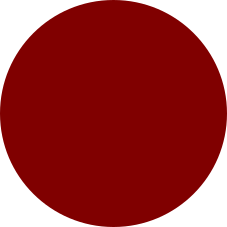
\includegraphics[width=2.5cm, height=2.5cm]{../images/figuras2d/circulo.png}
		}
		\subfigure[ Rombo]{
			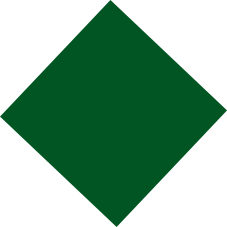
\includegraphics[scale=0.5]{../images/figuras2d/rombo.png}
		}
		\subfigure[ Pentagono]{
			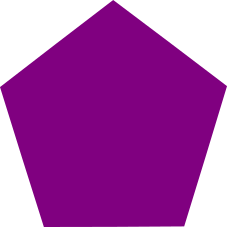
\includegraphics[scale=0.5, angle=45]{../images/figuras2d/pentagono.png}
		}
		\caption{Figuras geometricas de dos dimensiones}
	\end{figure}
\end{document}